\subsection{Classes}

With the elements described in the previous section, we can create a complete abstract graph search framework to be used in a wide variety of scenarios. As the decisions and content has been largely outlined already, each of the elements are easily translated into classes. All classes will be abstract except the \texttt{Result} class. As this class will contain a \texttt{State} and a boolean expressing if the search was successful.\footnote{Technically the \texttt{Result} could deliver the same information with only the \texttt{State} stating if the search was successes based on a null-check on the state. A boolean is kept in this implementation however, as the user may utilize null states in their system.} 

Many of the descriptions mentioned in the requirements will be implemented as abstract methods, where the functionality and search specifics are specified by the extending class. Simple or optional methods such as getters/setters or the link/heuristic methods are not forced to be overwritten, as multiple scenarios don't need these to be tailored.

The resulting classes are seen in figure \ref{fig:framwork_classdiagram}.

\begin{figure}[H]
    \centering
    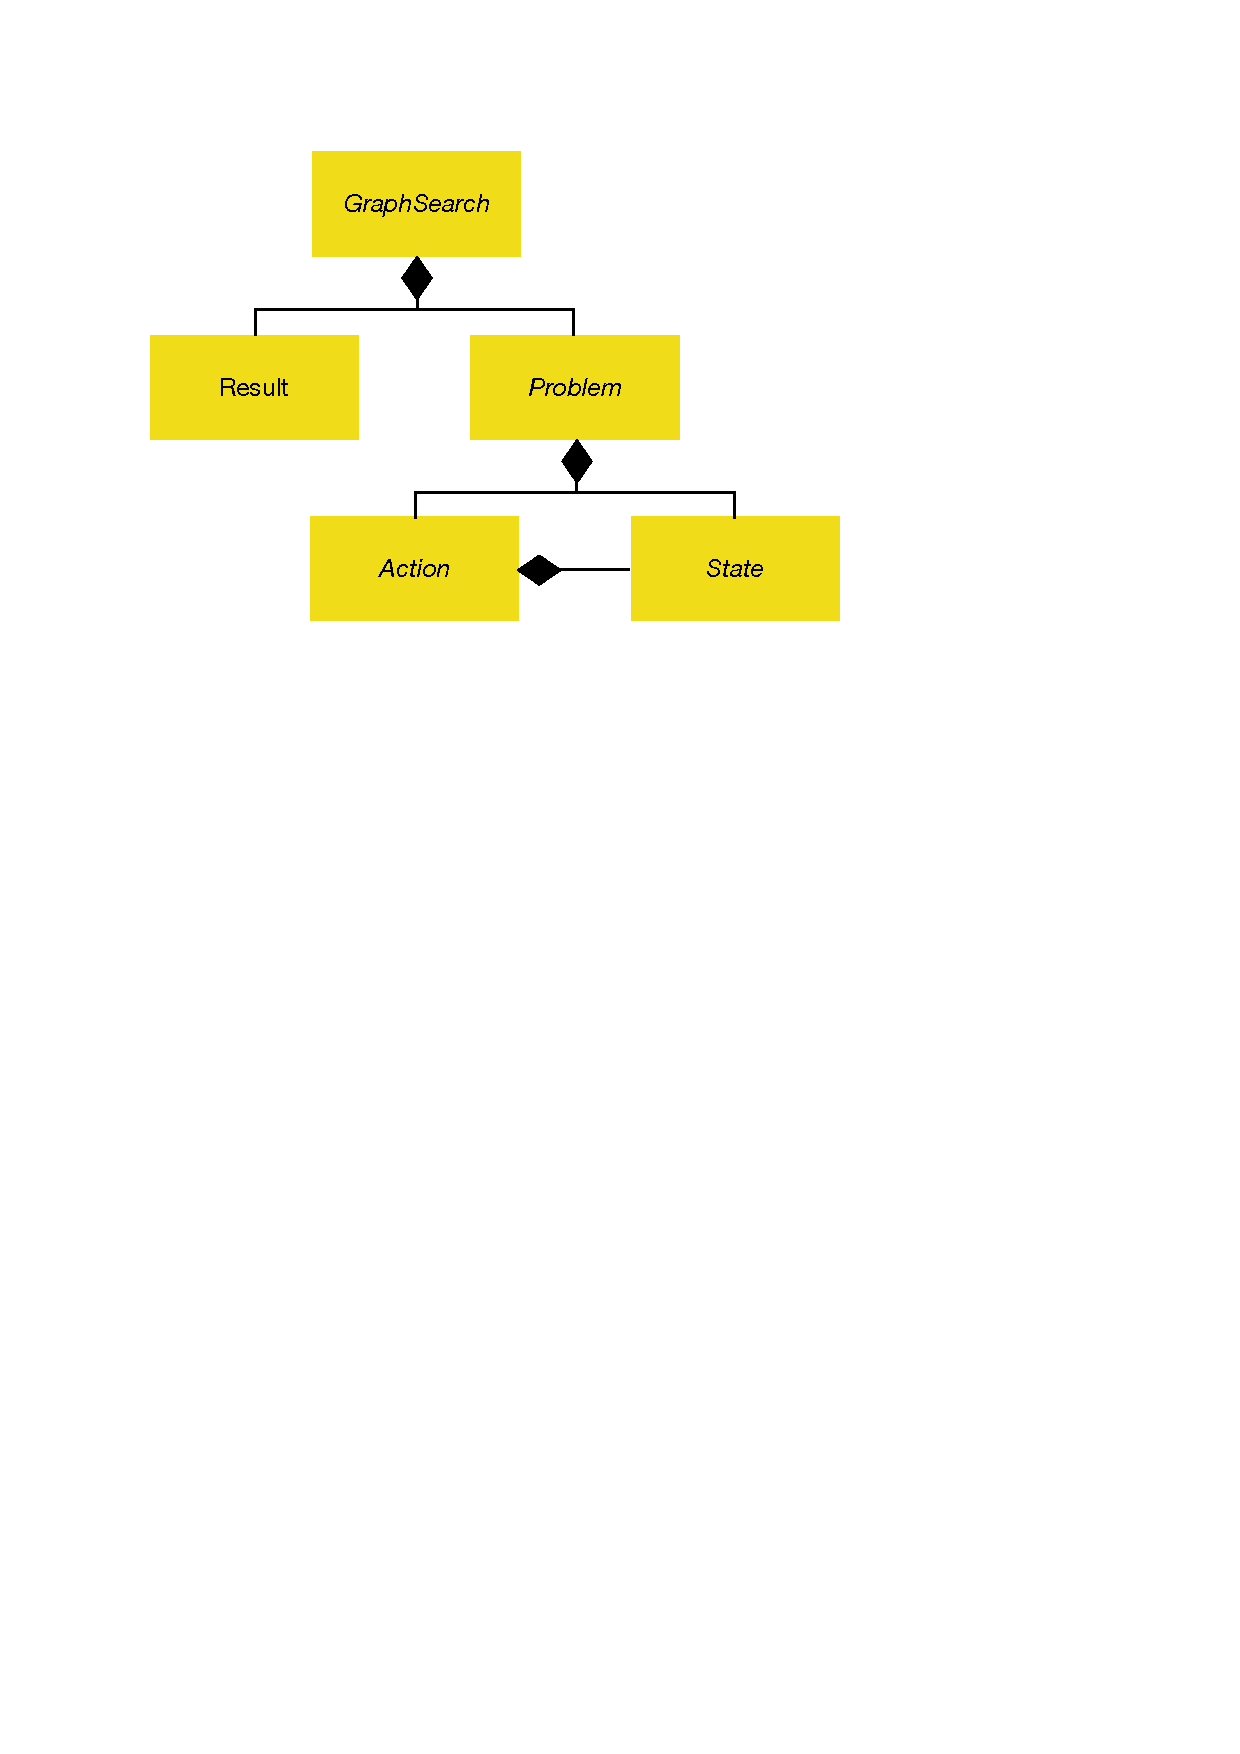
\includegraphics[width=0.6\linewidth]{FrameWork/AbstractFrameworkClassDiagram.pdf}
    \caption{Simple class diagram of the relationship between the framework classes.\protect\footnotemark}
    \label{fig:framwork_classdiagram}
\end{figure}

\footnotetext{Only the relations between the classes are shown in the class diagram to keep it clean, as the methods are described in the text above.}